\documentclass{exam}
\usepackage{graphicx} % Required for inserting images
\usepackage{listings}
\usepackage{amsmath}
\usepackage{algorithmicx}
\usepackage{algpseudocode}
\usepackage{geometry}[border=1in]
\usepackage{algorithm}
\usepackage{amsmath}
\usepackage{amssymb}
\usepackage{amsthm}
\usepackage{listings}
\usepackage{mathtools}
\usepackage{tikz}
\usetikzlibrary{arrows.meta,automata,positioning}

\newtheorem*{statement}{Statement}

\title{HW1 - DFA and Regular Languages}
\author{COMP361 --- Suhas Arehalli}
\date{Spring 2025}

\begin{document}
\maketitle

\section*{Instructions}
AS with previous homeworks, 

\begin{itemize}
    \item Deadlines are posted on the course website.
    \item Solutions should be turned in as a typeset pdf, preferably using LaTeX. I recommend a tool like overleaf. 
    \item Assignments are individual, and you should not share solutions with other students. However, you are free to discuss problems within the bounds of the academic integrity policy in the syllabus, and should indicate in your assignment the people you got assistance from (including instructors, peers, and preceptors!). 
    \item Proofread your work before submission, and consult the proof style guide to make sure your submissions are both correct and clear.
    \item Graded problems will be indicated by an asterisk (*) next to the problem number. You are still expected to solve all of the problems.
\end{itemize}

\section*{Questions}
\begin{questions}
    \question \textit{(Sipser 1.6bem)} For each of the following languages, prove that the language is regular by constructing a DFA that recognizes that language, presented as a 5-tuple. For each, the alphabet $\Sigma = \{0, 1\}$. You do \textbf{not} need to present a formal proof that the DFA does, in fact, recognize the language.
    \begin{parts}
        \part $L_1 = \{w \in \Sigma^* \mid w \text{ contains at least three 1s}\}$
        \part*$L_2 = \{w \in \Sigma^* \mid w \text{ begins with 0 and has odd length or begins with 1 and has even length}\}$
        \part $L_3 = \emptyset$
        \part $L_4 = \{\varepsilon\}$
    \end{parts}

    \question \textit{(Extending Sipser 1.6f)} Recall that in class, we defined $q \xrightarrow{w}_{M} q'$ to mean that, for a DFA $M = (Q, \Sigma, \delta, q_0, F)$ there exists a sequence of states $r_0, \dots, r_{\lvert w \rvert} \in Q$ such that (1) $r_0 = q$, (2) $r_i = \delta(r_{i-1}, w_i)$ for all $1 \leq i \leq n$, and (3) $r_{\lvert w \rvert} = q'$.  
    
    Consider the state diagram for the DFA $M_1$ in Fig. \ref{fig:M1}:

    \begin{figure}[h]
    \centering
    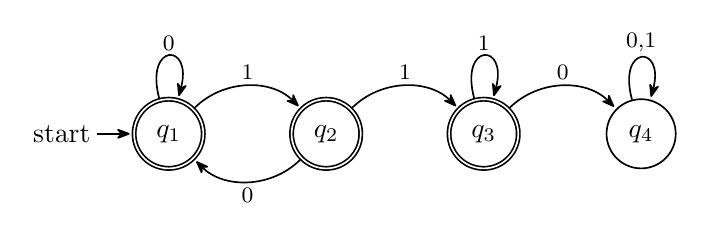
\begin{tikzpicture}[->,>={Stealth[round]},shorten >=1pt,
                    auto,node distance=2cm,on grid,semithick,
                    inner sep=2pt,bend angle=45]
    \node[initial,state,accepting]      (A)              {$q_1$};
    \node[accepting,state]              (B) [right=of A] {$q_2$};
    \node[accepting,state]              (C) [right=of B] {$q_3$};
    \node[state]                        (D) [right=of C] {$q_4$};

    \path [every node/.style={font=\footnotesize}]
        (A) edge [loop above] node {0} (A)
            edge [bend left]  node {1} (B)
        (B) edge [bend left ] node {0} (A)
            edge [bend left]  node {1} (C)
        (C) edge [loop above] node {1} (C)
            edge [bend left]  node {0} (D)
        (D) edge [loop above] node {0,1} (D)
        ;
    \end{tikzpicture}
        \caption{A state diagram for $M_1$}
        \label{fig:M1}
    \end{figure}
    \begin{parts}
        \part *Provide a formal definition of the DFA $M_1$ (i.e., a 5-tuple). 
        \part Prove that $q_4 \xrightarrow{w}_{M_1} q_4$ for all $w \in \Sigma^*$.  
        \part *Prove that $q' \xrightarrow{110}_{M_1} q_4$ for all $q' \in Q$.
        \part *Use the previous 2 parts to show that if 110 is a substring of $w$, $q_0 \xrightarrow{w}_{M_1} q_4$, and thus $w$ is rejected by $M_1$.
        \part Prove that if $q_1 \xrightarrow{w}_{M_1} q_4$, then 110 is a substring of $w$.
        \part *Use the prior parts to show that $M_1$ recognizes $A = \{w \in \Sigma^* \mid w \text{ does not contain the substring 110}\}$
    \end{parts}
\end{questions}

\end{document}

